\chapter{Standard Model}
\label{chap:sm}
The {SM} of particle physics is a quantum field theory that describes all
known fundemental constituents of matter and their interactions through the
strong, weak and electromagnetic forces.
The theory was pieced together in the 60s and 70s and comprises two families of
elementary particles, called quarks and leptons, and incorporates the theories
of quantum electrodynamics (QED), Glashow-Weinberg-Salam theory of electroweak
dynamics and quantum chromodynamics (QCD)
\cite{t1972regularization, glashow1961partial, weinberg1967model,
salam1968weak}.

The Standard Model is remarkable in its accuracy, describing every experimental
test performed.  
\todo[inline]{MAKE THIS GOODER.}

This chapter reviews the {SM} of particle physics. The first section will 
introduce the matter constituents of the standart model; the leptons and quarks,
and the latter section will describe the fundemental interactions. 
The description follows the example given in \cite{ral} with additional insights
from \cite{perkins2000introduction,griffiths2008introduction,halzen1984quarks}.

\section{Constituents of the Standard Model}
\label{sec:matter}
Within the Standard Model matter is described as being constructed from a small
number of spin$=\nicefrac{1}{2}$ particles called fermions that interact with
the electromagnetic, weak and strong forces. 
The fields corresponding to the the fermions are described by the dirac
equation,
\begin{equation}
\left( i \gamma^{\mu} \partial_{\mu} - m \right) \psi(x) = 0
\end{equation}
where $\psi(x)$ is a four-component spinor, $\gamma^{\mu}$ are the Dirac
matrices and $m$ is the fermion mass.

The fermions are divided in to two families called, leptons and quarks,
according to their experimentally measured properties such as their charge.
Each family of fermions can be further subdivided in to three generations that
increase progressively increase in mass. The fermions of the Standard Model and
some of their properties are summarised in \TableRef{tab:particles}.

\begin{table}[htbp]
\begin{center}
\begin{tabular}{l l l l l l }
\toprule
& 1st gen. & 2nd gen. & 3rd gen. & $Q$ & colour \\ 
\midrule
\multirow{2}{*}{quarks} 
& \Pup   & \Pstrange & \Ptop & $\nicefrac{+2}{3}$ & \multirow{2}{*}{$R,G,B$} \\
& \Pdown & \Pcharm   & \Pbottom & $\nicefrac{+2}{3}$ & \\ 
\multirow{2}{*}{leptons} 
& \Pnue      & \Pnum  & \Pnut & $0$ & \multirow{2}{*}{-} \\
& \Pelectron & \Pmuon & \Ptau & $1$ & \\ 
\bottomrule
\end{tabular}
\caption{The fermions of the Standard Model.}
\end{center}
\label{tab:particles}
\end{table}\todo{add particle masses?}

\subsection{Leptons}
Each lepton generation contains a charged lepton and a corresponding light
neutral particle called a neutrino.  For each leptron there is a corresponding 
anti-lepton with opposite charge, for example the positivly charged positron.
Therefore, in total there are 12 leptons.  All leptons interact via the weak
force, whereas only the charged leptons interact with the electromagnetic force.

The first generation of leptons is the most familiar containing the electron and
the electron neutrino.

\subsection{Quarks}
There are six flavours of quark arranged in to three generations.
Unlike leptons, quarks carry fractional charge, within each generation there is
a quark with a charge of $\nicefrac{2}{3}$ and another with a charge of
$\nicefrac{-1}{3}$. As well as the electric charge, quarks carry an additional
charge called the colour charge. The colour charge allows the quarks to interact
via the strong force in addition the electromagnetic and the weak forces.
For each quark, there is a corresponding anti-quark which has opposite charge
and colour charge. Including the anti-quarks there are a total of 12 quarks.

The first generation of quarks is again the most familiar, containing the up and
down type quarks that are the constituents of the proton and neutron, which in
turn, with the electron, form atoms and all familiar matter.

\section{Fundamental Forces}
\label{sec:forces}

There are, as far as is known, four fundemental forces of nature, the strong,
weak, electromagnetic and gravitational forces.
\TableRef{tab:forces} summarises the forces in order of decreasing
strength\footnote{The strength quoted in the table is a rough approximation as
`strength' depends on the source and distance of a
force\cite{griffiths2008introduction}}

\begin{table}[htbp]
\begin{center}
\begin{tabular}{ l l l l }
\toprule
Force           & Strength   & Theory   & Mediator \\
\midrule
Strong          & $10^{0}  $ & {QCD} & Gluon \\
Electromagnetic & $10^{-2} $ & {QED} & Photon \\
Weak            & $10^{-13}$ & {EWK} & \PW and \PZ \\
Gravitational   & $10^{-42}$ & General Theory of Relativity & Graviton? \\
\bottomrule
\end{tabular}
\caption{The known four fundemental forces \cite{griffiths2008introduction}.}
\end{center}
\label{tab:forces}
\end{table}

The {SM} describes the strong, weak and electromagnetic interactions. Each
force is mediated by exchange of integer spin intermediate particles called
bosons.
The boson constituent of the {SM} are summarised in \TableRef{}.

\begin{table}[htbp]
\begin{center}
\begin{tabular}{l l c c }
\toprule
name & mass & charge \\
\midrule
Photon (\Pphoton) & 0    & 0 \\
\PWpm             & 80.4 & $\pm1$ \\
\PZ               & 91.2 & 0 \\
gluon (\Pgluon)   & 0    & 0 \\
\bottomrule
\end{tabular}
\caption{The boson of the Standard Model.}
\end{center}
\label{tab:boson}
\end{table}

Gravity is not included in the {SM} as a complete quantum theory of gravity
has not yet been found. However, the gravitational force is very weak when
compared to the other three forces so its contribution to particle interactions
is negligable.

\subsection{QED}
The classical theory for electromagnetism was formulated by Maxwell over a
centuary ago\cite{maxwell}, and a quantum theory of electrodynamics was
realised by Tomonaga, Feynman and Schwinger in the 1940s \cite{qed}.

The {EM} force is the force that is responsible for interaction between
charged particles. The force is mediated by the massless photon, which means
that the {EM} force is effective over infinite range.
The fundemetal process of {QED} is shown in \FigureRef{fig:qed}.
\begin{figure}[htbp]
  \centering
  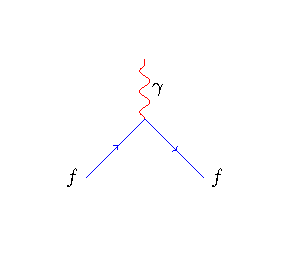
\includegraphics[width=0.5\textwidth]{qed_process}
  \caption{The elementary process for {QED} that all electromagnetic
interactions can be reduced to.}
  \label{fig:qed}
\end{figure}

The fine structure constant, $\alpha$, specifys the strength of the interaction
between charged particles and photon and is given by
\begin{equation}
\alpha = \frac{e^2}{4 \pi} \approx \frac{1}{137}
\end{equation}

The {SM} describes all the interactions of known particles in terms of gauge
theories. A gauge theory is a theory that is invariant under a set of local
transformations.  In electromagnetism the gauge transformations are local
complex phase transformations of the charge particle fields. Requiring gauge
invariance will in turn require that a massless vector particle be introduced,
the photon, that mediates the {EM} interaction.

The lagrangian densitry for a free Dirac field, $\psi$, is given by,
\begin{equation}
\mathcal{L} = i \bar{\psi} \gamma_{\mu} \partial^{\mu} \psi - m \bar{\psi}\psi .
\end{equation}
This Lagrangian is invariant under a `global' phase transformation of the
fermion field,
\begin{equation}
\psi(x) \to e^{iQ\omega} \psi(x), \quad \bar{\psi}(x) \to e^{iQ\omega}\bar{\psi}(x),
\label{eq:global}
\end{equation}
where $Q$ is the charge operator and $\omega$ is a global arbitrary parameter. 
The Lagrangian is said to exhibit global gauge invariance. 

The family of transformations, $R = e^{i \omega}$, forms the
abelian group $U(1)$ which is the group of all unitary $1\time1$ matrices.
Unitary refers to the property that $U^{-1} = {U}^{\dagger}$
Abelian refers to the property that all the elements in a
group commute, 
\begin{equation}
e^{-i\omega_1} 
e^{-i\omega_2} 
=
e^{-i\omega_2} 
e^{-i\omega_1} .
\end{equation}

If a infinitesimal group transformation is considered then 
\begin{equation}
\psi(x) 
\to e^{iQ\omega} \psi(x)
\approx (1+iQ\omega)\psi(x),
\end{equation}
and the Lagrangian is unchanged by the transformation.

Global transformations introduce a problem that making a transformation requires
that every space-time point to `know' about the transformation. It would be
preferable to require invariance under local transformations.
More generally, the \EquationRef{eq:global} can be rewritten as,
\begin{equation}
\psi(x) \to e^{i\omega(x)} \psi(x),
\label{eq:local}
\end{equation}
where $\alpha$ is now a function of the space time coordinate $x$. This is known
as a local phase transformation. The infinitesimal transformation now becomes,
\begin{equation}
\psi(x) 
\to e^{iQ\omega} \psi(x)
\approx (1+iQ\omega)\psi(x),
\end{equation}
However, under this transformation the
Lagrangian is no longer invariant. 

The gauge invariance can be restored if it is assumed that the fermion field
interacts with a vector field, called a gauge field and denoted $A_{\mu}$, with
an interaction,
\begin{equation}
-e\bar{\psi}\gamma^{\mu}A_{\mu}Q\psi
\end{equation}
where $A_\mu$ transforms under a gauge transformation as 
\begin{align}
-eQA_{\mu} \to & -eQ(A_{\mu}+\delta A_{\mu}(x)\\
           =   & -e Q A_{\mu} + Q \partial_{\mu} \omega (x)
\end{align}
and the new Lagrangian then becomes
\begin{align}
\mathcal{L} 
&= \bar{\psi}( i\gamma^{\mu} ( \partial_{\mu} +i e Q A_{\mu}) - m)\psi \\
&= \bar{\psi}( i\gamma^{\mu} D_{\mu} - m)\psi 
\end{align}
where the covariant derivative has been introduced,
\begin{equation}
D_{\mu} \equiv \partial_{\mu} - i e A_{\mu}.
\label{eq:covar_deriv}
\end{equation}
The vector field, $A_{\mu}$, couples with the electron, and can be identified as
the physical photon field. 

To complete the lagrangian a kinetic term for the photon field should be added
which is quadratic in the derivative of the field.
However, this term should not break the invariance under gauge trnasformations.
This is achieved by defining the field strength tensor, $F_{\mu\nu}$,
\begin{equation}
F_{\mu\nu}
= \partial_{\mu} A_{\nu} - \partial_{\nu} A_{\mu}.
\label{eq:fieldstrengthtensor}
\end{equation}
which is gauge invariant. Therefore and term constructed only out of 
 $F_{\mu\nu}$ may be added to the Lagrangian.
A suitable term is $\frac{1}{4} F_{\mu\nu} F^{\mu\nu}$ which is quadratic in the
derivative of the field while remaining gauge invariant,
\begin{equation}
\mathcal{L} = \frac{1}{4} F_{\mu\nu} F^{\mu\nu} + \bar{\psi}( i\gamma^{\mu} D_{\mu} - m)\psi 
\end{equation}

Local gauge invariance has been restored with the introduction of the photon
field. An interesting result is that the photon is required to be massless, as
the introduction of a mass term for the photon, for example a term $\propto
A_{\mu}A^{\mu}$, will break the gauge invariance.

\subsection{Quantum Chromodynamics}
\label{sec:QCD}
The strong force is the force responsible for the interaction between particles
that carry a colour charge, quarks and gluons. Unlike the electric charge, the
colour charge can have three posible values, conventionally called `red',
`green' and `blue' , as well as the corresponding anti colout charges
`anti-red', `anti-green' and `anti-blue'.
The fundemetal quark-gluon process of the strong force is shown in
\FigureRef{fig:qcd}.
\begin{figure}[htbp]
  \centering
  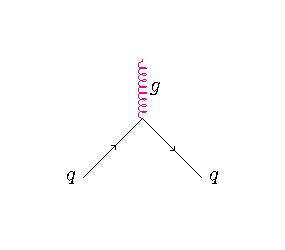
\includegraphics[width=0.5\textwidth]{qcd_process}
  \caption{The quark-gluon vertex for {QCD} .}
  \label{fig:qcdquark}
\end{figure}
The strong force is mediated by eight massless gluons which themselves carry
colour charge. This allows the gluons to self-interact which results gluon-gluon
vertexes in addtion to the quark-gluon vertex.

\begin{figure}[htbp]
  \centering
  \begin{subfigure}{0.45\textwidth}
    \centering
    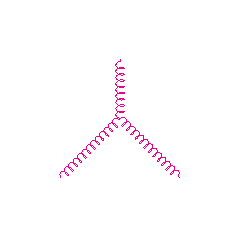
\includegraphics[width=\textwidth]{qcd_3gluon}
    \caption{Three-gluon vertex.}
    \label{fig:qcd_3gluon}
  \end{subfigure}
  \begin{subfigure}{0.45\textwidth}
    \centering
    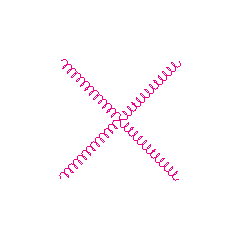
\includegraphics[width=\textwidth]{qcd_4gluon}
    \caption{Four-gluon process.}
    \label{fig:qcd_4gluon}
  \end{subfigure}
  \caption{Fundemental gluon-gluon vertices.}\label{fig:qcd_gluon} 
\end{figure}

The coupling constant for the strnog force, $\alpha_s$, is given by,
\begin{equation}
\alpha = \frac{g_s^2}{4 \pi} \approx 1
\end{equation}
which is approximately 100 times stronger than the {EM} force.
As the energy of the interaction increases the strength of the strong coupling
decreases. This is known as asymptotic freedom, at high-energy experiments
quarks appear to behave almost as free particles. However, at lower energies 
the coupling increases and quarks only appear in bound states, this is known as
quark confinement.
\todo{diagram of quark confinement here?}

The strong interaction is described by the theory of {QCD}.
Quantum chromodynamics follows from similar reasoning to the {QED} case, but with
the Abelian $U(1)$ symmetry group replaced with the non-Abelian $SU(3)$ symmetry
group of transformations on the quark colour fields.

\todo{show triplets here}
Quarks form colour triplets under $SU(3)$ transformations for each quark
flavour,

\begin{equation}
q_{f} =
\left(\begin{matrix} 
q^{red}_{f} \\
q^{green}_{f} \\
q^{blue}_{f} \\
\end{matrix} \right).
\end{equation}
The local gauge phase transformation under $SU(3)$,
\begin{equation}
q(x) \to e^{i\alpha_a(x)T_a} q(x),
\end{equation}
which breaks the invariance of the Lagrangian. Again this is overcome by
introducing the covariant derivative,
\begin{equation}
D_{\mu} \equiv \partial_{\mu} + i g T_{a} G_{\mu}^{a},
\end{equation}
where eight gauge fields have been introduced, instead of the single field in
QED. \todo{what is T} 
The gauge fields transform as,
\begin{equation}
 G_{\mu}^{a} \to G_{\mu}^{a} 
-\frac{1}{g}\partial_{\mu}\alpha_{a}
-f_{abc}\alpha_{b}G^{c}_{\mu},
\end{equation}
where last additional term has been added is to produce a gauge invariant
Lagrangian due to the non-Abelian gauge transformation.

The final Lagrangian for QCD can now be written,
\begin{equation}
\mathcal{L} = 
\bar{q}(i\gamma^{\mu}\partial_{\mu} - m)q -
g \bar{q} \gamma^{\mu} G_{\mu}^{a} - 
\frac{1}{4} G_{\mu\nu}^{a} G^{\mu\nu}_{a},
\end{equation}
where the field strength tensor $G^{\mu\nu}_{a}$ is given by,
\begin{equation}
G^{\mu\nu}_{a} 
= \partial{\mu} G^{a}_{\nu}
- \partial{\nu} G^{a}_{\mu}
-g f_{abc} G^{b}_{\mu} G^{c}_{\nu}.
\end{equation}

In a similar way to QED, the Lagrangian for interacting coloured quarks, $q$, and
vector gluons, $G_{\mu}$, result from the simple requirement of local colour
phase invariance of the quark fields. Unlike the QED case, eight gauge fields
are needed due to the three quark colour fields.  Similar to QED, the gluons are
required to  be massless.

The field strength tensor, $G^{\mu\nu}_{a}$, introduces terms that are cubic and
quadratic in $G$. These represent three and four vertex gluon interactions
(\FigureRef{fig:qcd_gluon}) that are a result of the non Abelian nature of the $SU(3)$ group.
 
\subsection{Weak Force}
The weak interaction occurs between all fermions and is the interaction
responsible in the radioactive decay of sub-atomic particles.  Unlike the strong
and electromagnetic forces, the weak force is mediated by the exchange of
massive particles, the \PWpm and \PZ bosons, which causes the weak interaction
to have a very short range.

There are two kinds of weak interactions: charged and neutral, mediated by the
\PW and the \PZ respectivly.

The fundemental vertex for the neutral vertex is shown in
\FigureRef{fig:neutral}, where the \PZ interacts with any quark or lepton.
The \PZ can mediate any process that can be mediated by the photon as well as
processes involving neutrinos.
\begin{figure}[htbp]
  \centering
  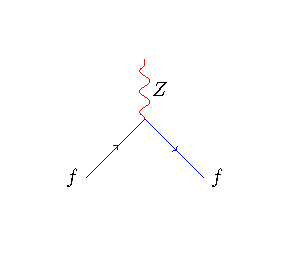
\includegraphics[width=0.5\textwidth]{weak_neut_process}
  \caption{The fundemental vertex of neutral weak vertex.}
  \label{fig:neutral}
\end{figure}

The fundemental vertices for the charged current are shown in
\FigureRef{fig:charged}. The charged current has the unique ability to chage the
flavour of quarks and leptons by the exchange of \PW bosons. The charged current
will only interact with fermions of the same generation
(\HepProcess{\Pelectron\to\Pnue} but never
\HepProcess{\Pelectron\to\Pnum}).

\begin{figure}[htbp]
  \centering
  \begin{subfigure}{0.45\textwidth}
    \centering
    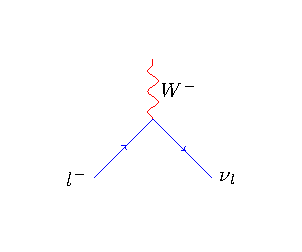
\includegraphics[width=\textwidth]{weak_charged_lepton_process}
    \caption{Leptons.}
    \label{fig:weak_charged_lepton_process}
  \end{subfigure}
  \begin{subfigure}{0.45\textwidth}
    \centering
    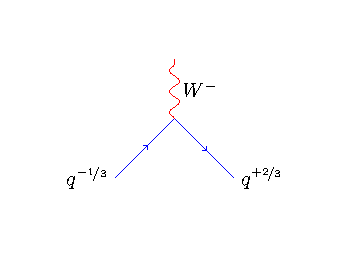
\includegraphics[width=\textwidth]{weak_charged_quark_process}
    \caption{Quarks.}
    \label{fig:weak_charged_quark_process}
  \end{subfigure}
  \caption{The fundemental vertices for charged weak vertex.}
  \label{fig:weak_charged}
\end{figure}

In a similar way to {QCD}, there are coupling of the \PW and \PZ to one
another as shown in \FigureRef{fig:weak_boson}.

\begin{figure}[htbp]
  \centering
  \begin{subfigure}{0.3\textwidth}
    \centering
    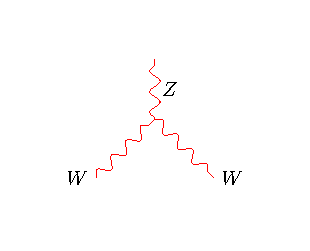
\includegraphics[width=\textwidth]{weak_WWZ}
    \caption{\HepProcess{\PW\PW\PZ}.}
    \label{fig:weak_WWZ}
  \end{subfigure}
  \begin{subfigure}{0.3\textwidth}
    \centering
    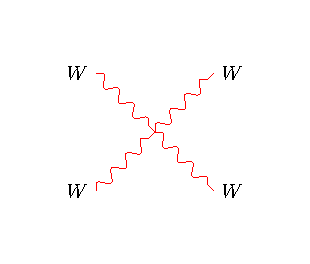
\includegraphics[width=\textwidth]{weak_WWWW}
    \caption{\HepProcess{\PW\PW\PW\PW}.}
    \label{fig:weak_WWWW}
  \end{subfigure}
  \begin{subfigure}{0.3\textwidth}
    \centering
    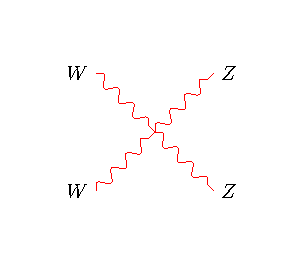
\includegraphics[width=\textwidth]{weak_WWZZ}
    \caption{\HepProcess{\PW\PW\PZ\PZ}.}
    \label{fig:weak_WWZZ}
  \end{subfigure}
  \caption{Direct couplings of the \PW and \PZ boson to each other.}
  \label{fig:weak_boson}
\end{figure}

The weak interaction also violates parity ($P$) and charge conjugation ($C$). A
well known example of parity violation in weak interactions is the Wu experiment
\cite{wu}. In the experiment the $\beta$ decay of nuclei (Cobalt-60) polarised by an
external magnetic is studied, 
\begin{equation}
\begin{matrix}
\Rightarrow\Rightarrow \\
^{60}\mathrm{Co} \\
~   
\end{matrix}
\to
{^{60}\mathrm{Ni}}
+
\begin{matrix}
\Rightarrow \\
\Pelectron \\
\leftarrow 
\end{matrix}
+
\begin{matrix}
\Rightarrow \\
\APnue \\
\rightarrow 
\end{matrix}
\end{equation}
The Cobalt-60 nuclei are aligned to the external magnetic field. By conservation
of angular momentum, the neutrino and electron spins must be parallel and
aligned with the magnetic field. By
momentum conservation, the electron and neutrino must be produced in opposite
directions which means that the electron and neutrino must have oposite helicity. 
By changing the direction of the magnetic field, the system undergoes a parity
transformation
\begin{equation}
\begin{matrix}
\Leftarrow\Leftarrow \\
^{60}\mathrm{Co} \\
~   
\end{matrix}
\to
{^{60}\mathrm{Ni}}
+
\begin{matrix}
\Leftarrow \\
\Pelectron \\
\leftarrow 
\end{matrix}
+
\begin{matrix}
\Leftarrow \\
\APnue \\
\rightarrow 
\end{matrix}
\end{equation}
If parity is conserved then the electron would have no preference in direction.
However, what was seen was that the electron was preferentially emitted in the
oppsoite direction to their spin, the weak interaction exhibits maximal parity
violation.
More generally, the \PWpm boson is unique in that it only interacts with left handed
particles (or right handed antiparticles).
The \PW and \PZ bosons also have 3 and 4 vertex couplings to each
another.\todo{refer to diagram this}

The electromagnetic and weak interactions can be described by a unified theory
known as the electroweak theory.

The gauge group for the electroweak theory is given by,
\begin{equation}
U(1)_{Y} \times SU(2)_{L} 
\end{equation}

The $L$ subscript on $SU(2)$ indicates that the weak force couples to the left
handed particles. 
The $Y$ indicates that the $U(1)$ group is not the gauge
group of QED but is that of the hypercharge which is connected to the electric
charge ($Q$) and the charge associated with the weak interaction, called weak
isospin ($I$), by the Gell-Mann-Nishikima relation,
\begin{equation}
Q = I_{3}+ \frac{1}{2}Y
\end{equation}

The next step is to write down the matter content of the theory. 
For the case of the leptons $l_{L}$ is a left
handed doublet,
\begin{equation}
l_{L} = \left( \begin{matrix} \nu \\ e \end{matrix} \right)_{L},
\end{equation}
and $e_{R}$ is a right handed singlet.
For the case of the quarks, $q_{L}$ is a left handed doublet,
\begin{equation}
q_{L} = \left( \begin{matrix} u\\ d \end{matrix} \right)_{L},
\end{equation}
and there are two right handed singlets, the $u_{R}$ and the $d_{R}$.
In this
description the left handed fermions form isospin doublets and the right
handed fermions are singlets. 
therefore under $SU(2)$ gauge transformations,
\begin{align}
e_{R} &\to e_{R}^{\prime} = e_{R}\\
l_{L} &\to l_{L}^{\prime} = e^{-i \omega^{a} \mathbf{T}^{a} }l_{L}
\end{align}
where, under $SU(2)$ transformations, the $SU(2)$ singlets are invariant so do
not couple with the corresponding gauge bosons.

The matter fields transform under the $U(1)_Y$ gauge transformations as,
\begin{equation}
\psi \to \psi^{\prime} = e^{-i\omega Y(\psi)}\psi
\end{equation}
where Y is the hypercharge of the particle.
\begin{equation}
Y(l_{L}) = -\frac{1}{2}, \qquad Y(e_{R}) = -1,
\end{equation}
\begin{equation}
Y(q_{L}) =  \frac{1}{6}, \qquad Y(u_{R}) =  \frac{2}{3}, \qquad Y(d_{R}) = -\frac{1}{3},
\end{equation}

The lagrangian for the electroweak interaction can be written as the sum of the
gauge boson and the fermion parts
\begin{equation}
\mathcal{L}_{electroweak} = 
\mathcal{L}_{fermion}
+ \mathcal{L}_{gauge}
\end{equation}


The fermion term has a lepton and a quark part.
\begin{equation}
\mathcal{L}_{fermion} =
 \mathcal{L}_{lepton}
+ \mathcal{L}_{quark}.
\end{equation}
The quark and lepton Lagrangians can be written by inspection of the general
expression in \EquationRef{eq:generallagrangian},
\begin{align*}
\mathcal{L}_{lepton} &= 
\bar{l}_{L} i \gamma^{\mu} \mathbf{D}_{\mu} l_{L} +
\bar{e}_{R} i \gamma^{\mu} D_{\mu} e_{R}, \\
\mathcal{L}_{quark} &= 
\bar{q}_{L} i \gamma^{\mu} \mathbf{D}_{\mu} q_{L} +
\bar{u}_{R} i \gamma^{\mu} D_{\mu} u_{R} +
\bar{d}_{R} i \gamma^{\mu} D_{\mu} d_{R},
\end{align*}
where the covariant derivative has been introduced.
The covariant derivative depends on the fermion field. The covariant derivative
for left-handed fermion, for example, is given by,
\begin{equation}
\mathbf{D}_\mu 
= \partial_\mu 
+ ig\mathbf{T}^{a}W_{\mu}^{a}
+ ig^{\prime}Y(l^{L})B_{\mu}
\end{equation}
where as the covariant derivative for the right-handed fermion, for example a
down quark, $d_R$,
\begin{equation}
D_\mu = \partial_\mu + ig^{\prime}Y(d^{R})B_{\mu}
\end{equation}
where $g^\prime$ and $g$ and are the two coupling constantsa and
$\mathbf{T}^{a}$ are the three generators of $SU(2)$ group.

The gauge part of the Lagrangian contains the kinetic terms and self interaction
terms for the gauge fields. By inspection of the general expression in
\EquationRef{eq:generallagrangian},
\begin{equation}
\mathcal{L}_{gauge} = 
- \frac{1}{4} B_{\mu\nu} B^{\mu\nu}
- \frac{1}{4} W^{a}_{\mu\nu} W^{a~\mu\nu}
\end{equation}
where the first term contains the hypercharge field strength and the second term 
contains the $SU(2)$ field stregth, so the index, $a$, runs from 1 to 3.
\begin{align*}
B^{\mu\nu}     &= \partial^{\mu} B^{\nu} - \partial^{\nu} B^{\mu},\\
W_{a}^{\mu\nu} &= \partial^{\mu} W_{a}^{\nu} - \partial^{\nu} W_{a}^{\mu} 
                + g \epsilon_{abc} W_{b}^{\mu} W_{c}^{\nu}.
\end{align*}

Several gauge fields have been introduced, eight gluon fields $G^{a}_{\mu}$;
three fields, $\mathbf{W}_{\mu}$ , corresponding to the $SU(2)_{L}$
group and a single gauge field, $B_{\mu}$, corresponding to the $U(1)_{Y}$ group.
The physical $\PWp$ and $\PWm$ bosons are superpositions of the $W^{1}_{\mu}$
and $W^{2}_{\mu}$ gauge fields
\begin{equation}
W^{\pm}_{\mu} = \frac{1}{\sqrt{2}} \left(W^{1}_{\mu} \mp W^{1}_{\mu}\right),
\label{eq:wgauge}
\end{equation}
and the photon and Z boson are combinations of the $B_{\mu}$ and $W^{3}_{\mu}$
gauge fields,
\begin{equation}
\left( \begin{matrix} A_{\mu}\\ Z_{\mu}\end{matrix}\right) =
\left( \begin{matrix} \cos\theta_{W} && \sin\theta_{W} \\  
                      -\sin\theta_{W} && \cos\theta_{W} \end{matrix}\right) 
\left( \begin{matrix} B_{\mu}\\ W^{3}_{\mu}\end{matrix}\right) ,
\label{eq:bgauge}
\end{equation}
where $\theta_{W}$ is the Weinberg angle which is related to the coupling
constants by
\begin{align*}
\sin\theta_{W} &= \frac{g\prime}{\sqrt{g^{2}+g\prime^{2}}},\\
\cos\theta_{W} &= \frac{g}{\sqrt{g^{2}+g\prime^{2}}}.
\end{align*}

\subsubsection{Higgs}

The Lagrangian, as it has been written so far, does not include terms for the
mass of any of the particles.  Adding in mass terms by hand will break the gauge
symmetry rendering the theory meaningless.  \todo[inline]{WHY!}

The symmetry needs to be broken in some natural way.  Spontaneous Symmetry
Breaking is a method to break the symmetry by requiring that the Lagrangian of a
system remains invariant under a transformation, but the ground state is not
invariant.

An example of {SSB} is a point mass in a potential,
\begin{equation}
V(r) = \mu^{2} \vec{r} \cdot \vec{r} + \lambda ( \vec{r} \cdot \vec{r} )^{2}
\end{equation}
where $\lambda$ is positive. This potential is symmetric. 

A point mass sits at $\vec{r}=0$. If $\mu^{2}>0$, as shown in
\FigureRef{higgs_pot_mup} then $\vec{r}=0$ is the ground state and
the mass will remain at this point.
If $\mu^{2}<0$ then the potential will look like that given in
\FigureRef{fig:higgs_pot_mum}. The system remains symmetric, but $\vec{r}=0$ is no longer
the ground state. To fall to the ground state the mass has to ``choose'' a
direction to fall. The choice will break the symmetry of the system, the
potential remains symmetric, but the ground state is not. This is an example of
{SSB}.

\begin{figure}[htbp]
  \centering
  \begin{subfigure}{0.45\textwidth}
    \centering
    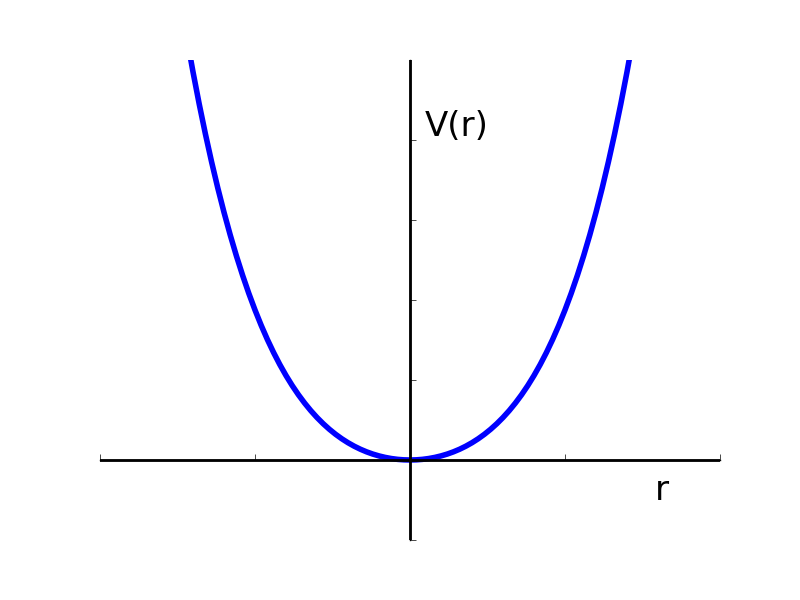
\includegraphics[width=\textwidth]{higgs_pot_mup}
    \caption{$\mu^{2}>0$.}
    \label{fig:higgs_pot_mup}
  \end{subfigure}
  \begin{subfigure}{0.45\textwidth}
    \centering
    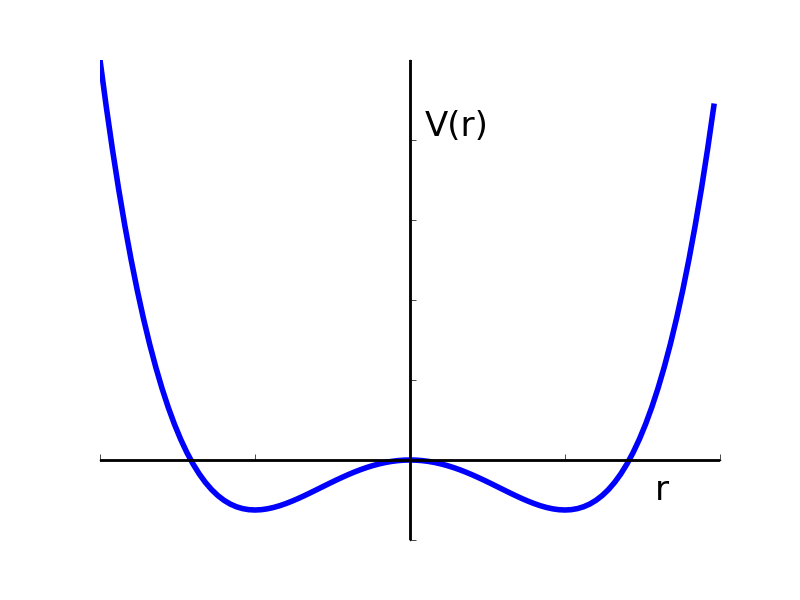
\includegraphics[width=\textwidth]{higgs_pot_mum}
    \caption{$\mu^{2}<0$.}
    \label{fig:higgs_pot_mum}
  \end{subfigure}
  \caption{The potential $ V(r) = \mu^{2} \vec{r} \cdot \vec{r} + \lambda (
\vec{r} \cdot \vec{r} )^{2}$.}
  \label{fig:higgs_pot}
\end{figure}

The application of {SSB} to the {SM} was studied by Higgs, Englert, Brout
and others \cite{higgs1981broken, englert1964broken, guralnik1964global}.
The result was a mechanism that spontaneous breaks the
 $SU(2)_{L} \times U(1)_{Y}$ symmetry called the Higgs mechanism\footnote{or the
Brout-Englert-Higgs mechanism, or even the
Englert-Brout-Higgs-Guralnik-Hagen-Kibble mechanism.}.

The Higgs mechanism introduces four real scalar fields, that can be arranged in a
doublet under $SU(2)$,
\begin{equation}
\Phi = \left( \begin{matrix} \phi^{+} \\ \phi^{0} \end{matrix} \right),
\end{equation}
where,
\begin{align*}
\phi^{+} &=\frac{1}{\sqrt{2}} (\phi_{1} + i \phi_{2}),\\
\phi^{0} &=\frac{1}{\sqrt{2}} (\phi_{3} + i \phi_{4}).
\end{align*}
The additional scalar part of the Lagrangian is,
\begin{equation}
\mathcal{L}_{scalar} = 
\left(D^{\mu}\Phi\right) \left(D_{\mu}\Phi\right) - V(\Phi),
\end{equation}
where the potential is,
\begin{equation}
V(\Phi) = 
\mu^{2}\Phi^{\dagger}\Phi + 
\lambda^{2} \left( \Phi^{\dagger} \Phi \right)^{2},
\end{equation}
where $\lambda$ and $\mu$ are free parameters. This lagrangian is invariant
under $SU(2)_{L} \times U(1)_{Y}$ transformations.
By choosing  $\lambda>0$ and
$\mu^{2}<0$ there is a minima at,
\begin{equation}
\Phi^{\dagger} \Phi = \frac{- \mu^{2}}{2 \lambda}.
\end{equation}
A plot of the Higgs potential with $\mu^{2}<0$ is shown in
\FigureRef{fig:higgspot}. It is unstable to small perturbations, and will fall
to a lower energy state. 

The ground state does not have the same symmetry as the Lagrangian; by
selecting a minima the symmetry has become broken. An example choice of minima
could be,
\begin{equation}
\phi_{1} = \phi_{2} = \phi_{4} = 0,
\end{equation}
and
\begin{equation}
\phi_{3} = \frac{-\mu^{2}}{\lambda} \equiv v^{2}.
\end{equation}
which leaves results in a non-zero {vev},
\begin{equation}
<0|\Phi|0> = \frac{1}{\sqrt{2}}\left(\begin{matrix}0\\v\end{matrix}\right),
\end{equation}

$\Phi$ can then be expanded around the vacuum minimum in terms of the four real
field $H$ and $\phi_1$, $\phi_2$ and $\phi_3$.
\begin{equation}
\Phi = 
\frac{1}{\sqrt{2}}
e^{i\nicefrac{\sigma}{2}\phi_a}
\left(\begin{matrix}0\\v+H\end{matrix}\right)
\approx 
\frac{1}{\sqrt{2}}
\left(\begin{matrix}0\\v+H\end{matrix}\right)
\end{equation}
where the $SU(2)$ invariance of the lagrangian allows for the choice of $\phi_i$
to be zero\cite{halzen1984quarks}.

The Lagrangian can be now written in terms of the $H$ field. The kinetic
term,\cite{ral}
\begin{align}
\left(D_{\mu}\Phi\right) \left(D^{\mu}\Phi\right) 
= \frac{1}{2} \left(\partial_{\mu}H\right) \left(\partial^{\mu}H\right)
+ \frac{g^{2}v^{2}}{4} W_{\mu}^{+} W^{-~\mu}
+ \frac{g^{2}v^{2}}{8 \cos^{2}\theta_{W}} Z_{\mu} Z^{\mu}
+ 0 A_{\mu} A^{\mu}
+ \text{~ interaction terms},
\end{align}
now includes mass terms for the gauge bosons,
\begin{equation}
M_{W} = \frac{1}{2}gv, \qquad 
M_{Z} = \frac{1}{2}\frac{gv}{8\cos^{2}\theta_{W}} .
\end{equation}
while the photon remains massless, $M_{A}=0$.

\subsubsection{Fermion Masses and Yukawa Couplings}

Another feature of the Higgs mechanism, is that it also provides a way to
introduce mass terms for the fermions, in a gauge invariant way, via the Yukawa
coupling between the leptons with the Higgs field. The Lagrangian for this
interaction for the electron can be written as, 
\begin{equation}
\mathcal{L}_{yukawa} = -Y_{e}\bar{l}_L\Phi e_R + h.c. \ ,
\end{equation}
where $Y_{e}$ is the coupling to the Higgs field known as the Yukawa coupling
and h.c. stands for hermitian conjugate. On substitution of $\Phi$ (from
\EquationRef{}), the lagrangian for the Yukawa couplings becomes
\begin{equation}
\mathcal{L}_{yukawa} = 
-\frac{Y_{e}}{\sqrt{2}} v
(\bar{e}_L e_R + \bar{e}_R e_L)
-\frac{Y_{e}}{\sqrt{2}}
(\bar{e}_L e_R + \bar{e}_R e_L)H
\end{equation}
and if $G_e$ is chosen such that
\begin{equation}
m_{e} = \frac{G_{e}v}{\sqrt{2}}
\end{equation}
then the lagrangian simplifies to
\begin{equation}
\mathcal{L}_{yukawa} = 
- m_e \bar{e}e
- \frac{m_e}{v} \bar{e}e H
\end{equation}
which represents a mass term for the electron and a coupling of the electron to
the Higgs field proportional to the mass of the electron.
The quark masses can also be generated in a similar way \cite{halzen}.

\todo[inline]{should I include a point here about the higgs boson itself and
then link it to the discovery?}
\cite{aad2012observation} and \cite{chatrchyan2012observation}
\todo[inline]{summarise the main points of this section}

